\documentclass{standalone}
\usepackage{graphicx}	
\usepackage{amssymb, amsmath}
\usepackage{color}

\usepackage{tikz}
\usetikzlibrary{intersections, backgrounds, math}
\usepackage{pgfmath}

\definecolor{light}{RGB}{220, 188, 188}
\definecolor{mid}{RGB}{185, 124, 124}
\definecolor{dark}{RGB}{143, 39, 39}
\definecolor{highlight}{RGB}{180, 31, 180}
\definecolor{gray10}{gray}{0.1}
\definecolor{gray20}{gray}{0.2}
\definecolor{gray30}{gray}{0.3}
\definecolor{gray40}{gray}{0.4}
\definecolor{gray60}{gray}{0.6}
\definecolor{gray70}{gray}{0.7}
\definecolor{gray80}{gray}{0.8}
\definecolor{gray90}{gray}{0.9}
\definecolor{gray95}{gray}{0.95}

\tikzmath{
  function mu(\x) {
    return 6 + -0.1 * \x - 0.01 * \x * \x + 0.003 * \x * \x * \x;
  };
}

\begin{document}

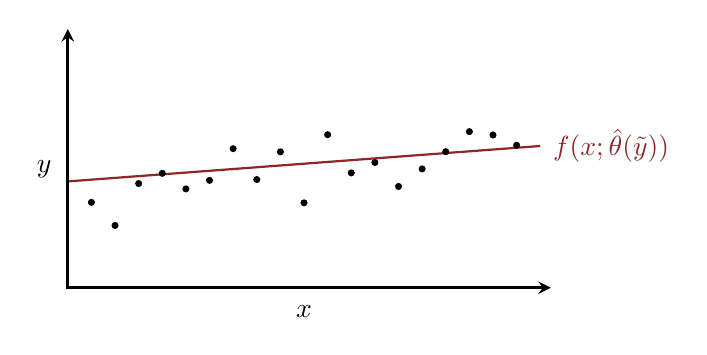
\begin{tikzpicture}[scale=0.3, thick]
  \draw[color=dark] (-10, 4.5) -- (10, 6);
  \node[color=dark] at (13, 6) { $f(x; \hat{\theta}(\tilde{y}))$ };

  %  Data simulated from f(x) = 0.075 * x + 5.25
  \foreach \y [count=\x from -9] in {3.613583, 2.636109, 4.409468, 4.842223, 4.184263, 4.544689, 5.886989, 
                                     4.580178, 5.752418, 3.593067, 6.478150, 4.862955, 5.300252, 4.286607, 
                                     5.030374, 5.758290, 6.608015, 6.463606, 6.028728} {
    \fill [fill=black] (\x, \y) circle (0.15);   
  }

  \draw [->, >=stealth, line width=1] (-10.05, 0) -- +(20.5, 0);
  \draw [->, >=stealth, line width=1] (-10, -0.05) -- +(0, 11);
  \node[] at (0, -1) { $x$ };
  \node[] at (-11, 5) { $y$ };
  
  
  
\end{tikzpicture}

\end{document}  